\documentclass[12pt]{article}%

\usepackage{fancyhdr}
\pagestyle{fancy}
\fancyhf{}
\fancyhead[R]{\thepage}

\usepackage{cmap}				
\usepackage{mathtext} 
\usepackage{listings}

\usepackage{biblatex}
\addbibresource{lib.bib}

\usepackage{euscript}
\usepackage{mathrsfs}

\usepackage[T2A]{fontenc}
\usepackage[utf8]{inputenc}
\usepackage[english,russian]{babel}
\usepackage{amsmath,amsfonts,amssymb,amsthm,mathtools}

\setlength\fboxsep{3pt}
\setlength\fboxrule{1pt}

% Работа с графикой и рисунками
\usepackage{graphicx} 
\usepackage{subcaption}

\usepackage{hyperref}
\usepackage[usenames,dvipsnames,svgnames,table,rgb]{xcolor}
\usepackage{wrapfig}
\hypersetup{				
    unicode=true,           
    pdftitle={Заголовок},   
    pdfsubject={Тема},      
    pdfkeywords={keyword1} {key2} {key3},
    colorlinks=true,
    linkcolor=black,
    citecolor=black,
    filecolor=magenta,
    urlcolor=cyan
}

% Работа с Python
\usepackage{minted}
\definecolor{LightGray}{gray}{0.98}

% Работа с enumerate
\usepackage{enumitem}

\newcommand*{\Title}{\begingroup
\centering 

\large {Федеральное автономное образовательное учреждение высшего образования}
\vspace*{\baselineskip}

\large {«Национальный исследовательский университет «Высшая школа экономики»»}
\vspace*{\baselineskip}

\vspace*{\baselineskip}
\large{\textbf{Отчет по лабораторной работе 5}}

\vspace{0.1cm}
\large{Минимизация функций}

\vspace{0.2cm}
\large{Вариант 10: задачи 9.1.10, 9.2.4, 9.5.10, 9.6.10}

\vspace{1.5cm} 

\begin{flushright}
  \textbf{\normalsize Выполнил:}
  
  \vspace{0.3cm} 
  {\normalsize Студент группы БПМ-211}
  
  {\normalsize Ляхов Артём Андреевич}

\end{flushright}


\vspace{0.2cm}  
\begin{flushright}
  \textbf{\normalsize Преподаватель:} 

  \vspace{0.2cm}

 {\normalsize Брандышев Петр Евгеньевич}
 
\end{flushright}

\vfill
\date{}{Май 2024 г.}


\endgroup\clearpage}

\begin{document}
\Title
\tableofcontents

\newpage

\section{Задача 9.1.10. Минимум и максимум унимодальной функции на отрезке}
\subsection{Формулировка задачи}
Необходимо методом Ньютона найти минимум и максимум унимодальной на отрзке $[a, b]$ функции $f(x)$ с точностью до $\varepsilon = 10^{-6}$. Предусмотреть подсчёт количества итераций, потребовавшихся для достижения заданной точности.

Согласно условию варианта:
\[
f(x) = e^x \cdot \cos{x}\ \ \ \ \ \ [a, b] = [0, 1.5]
\]

\subsection{Теоретический материал}
Предположим, что нам дана дважды непрерывно-дифференцируемая функция $f: \mathbb{R} \rightarrow \mathbb{R}$ и мы решаем задачу оптимизации:
\[
f(x) \rightarrow extr
\]
Пусть $x_{k}$ - $k$-ое приближение экстремума. Воспользуемся разложением функции $f(x)$ в окрестности точки $x_{k}$:
\[
f(x_k + t) \approx f(x_k) + f'(x_k)t + \frac{1}{2}f''(x_k)t^2
\]
Определим следующую итерацию так, чтобы функция достигала экстремума в $x_{k} + t$ и установим $x_{k+1} = x_{k} + t$. Для этого необходимо найти производную функции $f(x_k + t)$ по $t$ и приравнять её к нулю. Заменив $f(x_k + t)$ квадратичной аппроксимацией мы получаем следующее уравнение:
\[
\frac{d}{dt}\left(
f(x_k) + f'(x_k)t + \frac{1}{2}f''(x_k)t^2
\right) = 
f'(x_k) + t \cdot f''(x_k) = 0 
\]
Отсюда мы получаем итерационный метод, который называется методом Ньютона:
\begin{equation}
    x_{k + 1} = x_{k} - \frac{f'(x_k)}{f''(x_{k})}
\end{equation}

Существенным недостатком метода Ньютона является то, что в общем случае он сходится к стационарной точке и не позволяет определить является ли полученная точка максимумом или минимумом. Одним из способ проверить это является вычисление второй производной. Если $x^*$ - стационарная точка и $f''(x^*) < 0$, то $x^*$ - локальный максимум, если же $f''(x^*) > 0$, то локальный минимум.

Таким образом, чтобы найти максимум или минимум унимодальной функции на отрезке нам будет необходимо с помощью метода Ньютона найти стационарную точку $x^*$, проверить значение $f''(x^*)$, а также рассмотреть значения функции на границах отрезка.

\subsection{Результаты}
\begin{figure}[!h]
    \centering
    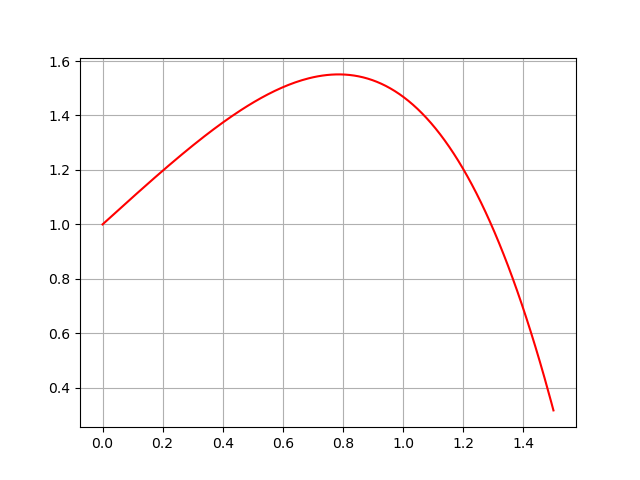
\includegraphics[width=\textwidth]{task1_plot.png}
    \caption{График функции $f(x) = e^x \cdot \cos(x)$ на отрезке $[0, 1.5]$}
\end{figure}

Как мы можем видеть из рисунка, точка максимума является внутренней точкой отрезка, и чтобы найти его можно воспользоваться методом Ньютона, при этом минимум достигается в одной из граничных точек отрезка.

В таблице ниже представлены результаты применения метода Ньютона к нашей задаче.

\begin{table}[!h]
\centering
\begin{tabular}{|c|c|c|c|}
    \hline Итераций & $x_{max}$ & $f(x_{max})$ & $f''(x_{max})$  \\
    \hline 4 & 0.785398 & 1.550883 & -3.101766 \\
    \hline
\end{tabular}
    \caption{Результаты нахождения точки максимума функции $f(x)$ с точностью $\varepsilon = 10^{-6}$ с помощью метода Ньютона. Поскольку $f''(x_{max}) < 0$, то найденная точка действительно является локальным, а следовательно в силу квазивогнутости $f(x)$ и глобальным, максимумом функции на отрезке.}
\end{table}

\begin{table}[!h]
    \centering
    \begin{tabular}{|c|c|c|}
    \hline x & a=0 & b=1.5  \\
    \hline f(x) & 1.0 & 0.317022 \\
    \hline
    \end{tabular}
    \caption{Значения $f(x)$ в границах отрезка. Поскольку $f(b) < f(a)$, то $x_{min} = b = 1.5$ - точка минимума функции на отрезке.}
\end{table}


\begin{table}[!h]
    \centering
    \begin{tabular}{|c|c|c|}
\hline & $x_{min}$ & $x_{max}$  \\
\hline $x$ & 1.5 & 0.785398 \\
\hline $f(x)$ & 0.317022 & 1.550883 \\
\hline
    \end{tabular}
    \caption{Минимум и максимум функции $f(x)$ на отрезке $[a, b]=[0, 1.5]$}
    \label{tab:my_label}
\end{table}

\newpage
\begin{figure}[!h]
    \centering
    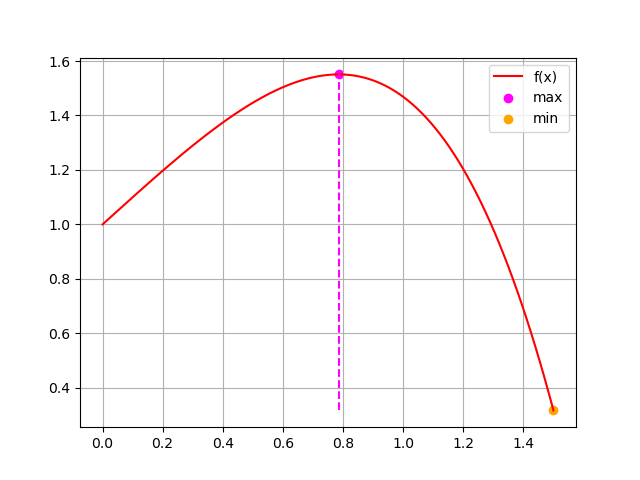
\includegraphics[width=0.95\textwidth]{task1_opt.png}
    \caption{Визуализация минимума и максимума функции на отрезке.}
\end{figure}



\subsection{Код на Python}
\begin{minted}[
frame=single,
framesep=10pt,
framerule=0.1pt,
bgcolor=LightGray
]{python}
def newton_optimize(
    func: Callable[float, float],
    func_der1: Callable[float, float],
    func_der2: Callable[float, float],
    x0: float,
    eps: float = 1e-6, 
    max_iter: int = 2500) -> tuple[float, int]:
    """
    Finds the extremum of a function using Newton method.
    """
    if np.isclose(func_der2(x0), 0.0):
        raise ValueError("f''(x0) = 0.0")

    x1 = x0 - func_der1(x0)/func_der2(x0)
    n_iter = 1

    while np.abs(x1 - x0) > eps and n_iter < max_iter:
        x0 = x1
        x1 -= func_der1(x1) / func_der2(x1)
        n_iter += 1

    return x1, n_iter
\end{minted}


\newpage
\section{Задача 9.2.4. Нахождение экстремума функции с помощью метода золотого сечения}
\subsection{Формулировка задачи}
Указананным в индивидуальном варианте методом найти минимумы и максимумы функции $f(x)$ на отрезке $[x_1, x_2]$ с точностью $\varepsilon=10^{-6}$. Предусмотреть подсчет числа итераций, потребовавшихся для достижения 
заданной точности.

Согласно варианту необходимо использовать \textit{метод золотого сечения} и при этом:
\[
f(t) = \frac{t^2 - t - 1}{t^2 + t + 5}\ \ \ \ \ [x_1, x_2] = [-1, 2]
\]

\subsection{Теоретический материал}
Пусть $f(x)$ - унимодальная непрерывно-дифференцируемая на отрезке $[a, b]$ функция. Одним из методом поисках минимума и максимума $f(x)$ на отрезке является \textit{метод золотого сечения} который состоит из следующих шагов: 
\begin{enumerate}
    \item Задаются начальные границы отрезка $[a, b]$, точность $\varepsilon$.
    \item Расчитываются точки деления $x_1 = b - \frac{(b - a)}{\phi}$, 
    $x_2 = a + \frac{(b - a)}{\phi}$, где $\phi = \frac{\sqrt{5} + 1}{2}$, и значения в них целевой функции $y_1 = f(x_1)$, $y_2 = f(x_2)$
    \item Если $y_1 \ge y_2$ (для поиска максимума - $y_1 \le y_2$), то $a = x_1$, в противном случае $b = x_2$.
    \item Если $|b - a| < \varepsilon$, то  $ x = \frac{1}{2}(a + b)$ и остановка. В противном случае возвращаемся к шагу 2. 
\end{enumerate}

\newpage
\subsection{Результаты}
\begin{figure}[!h]
    \centering
    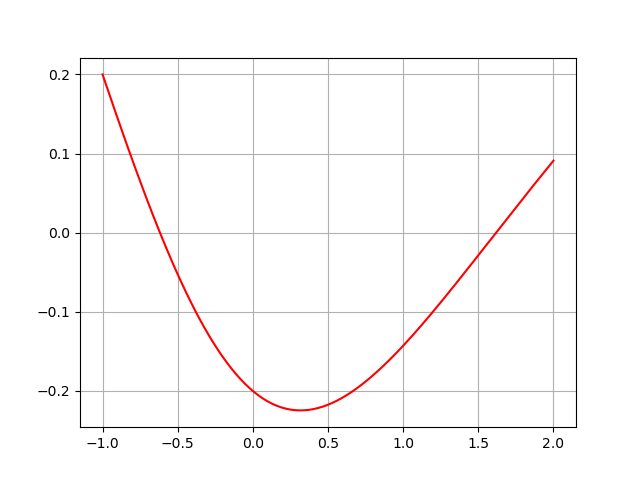
\includegraphics[width=0.8\textwidth]{task2_plot.png}
    \caption{График функции $f(x)$ на отрезке $[-1, 2]$.}
\end{figure}

Как мы видим, рассматриваемая функция имеет единственную точку минимума на отреке, а максимум функции достигается в одной из границ отрезка.

\begin{table}[!h]
\centering
\begin{tabular}{|c|c|c|}
    \hline Итераций & $x_{min}$ & $f(x_{min})$ \\
    \hline 31 & 0.316625 & -0.224553 \\
    \hline
\end{tabular}
    \caption{Результаты нахождения минимума $f(x)$ на отрезке с точностью $\varepsilon=10^{-6}$ с помошью метода золотого сечения.}
\end{table}

\begin{table}[!h]
    \centering
    \begin{tabular}{|c|c|c|}
    \hline x & a=-1.0 & b=2.0  \\
    \hline f(x) & 0.2 & 0.090909 \\
    \hline
    \end{tabular}
    \caption{Значения $f(x)$ в границах отрезка.}
\end{table}

\newpage
\begin{table}[h]
    \centering
    \begin{tabular}{|c|c|c|}
\hline & $x_{min}$ & $x_{max}$  \\
\hline $x$ & 0.316625 & -1.0 \\
\hline $f(x)$ & -0.224553 & 0.2 \\
\hline
    \end{tabular}
    \caption{Минимум и максимум функции $f(x)$ на отрезке $[a, b]=[-1, 2]$}
    \label{tab:my_label}
\end{table}

\begin{figure}[!h]
    \centering
    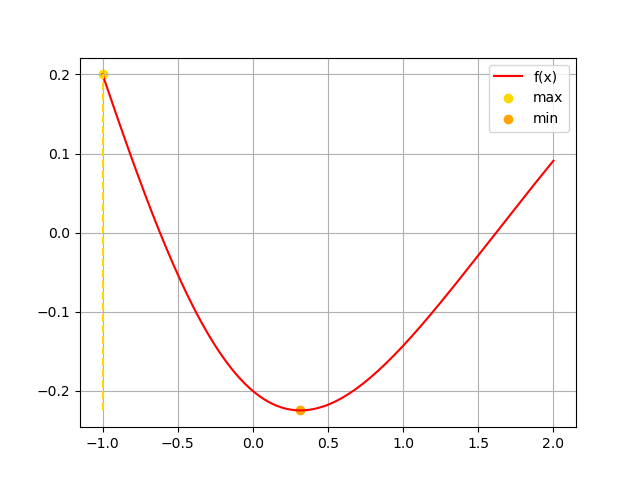
\includegraphics[width=0.7\textwidth]{task2_opt.png}
    \caption{Визуализация найденных минимума и максимума функции на отрезке: график $f(x)$ на отрезке $[a, b]$ вместе с точками $x_{min}$, $x_{max}$.}
\end{figure}

\subsection{Код на Python}
\begin{minted}[
frame=single,
framesep=10pt,
framerule=0.1pt,
bgcolor=LightGray
]{python}
from scipy.constants import golden_ratio


def golden_search(func, bounds, eps=1e-6):
    """
    Finds minimum of unimodal function on the 
    specified segment using golden search method.
    """
    a, b = bounds
    tau = golden_ratio
    n_iter = 0

    while np.abs(a - b) > eps:
        x1 = b - (b - a) / tau
        x2 = a + (b - a) / tau

        y1 = func(x1)
        y2 = func(x2)

        if y1 >= y2:
            a = x1
        else:
            b = x2

        n_iter += 1

    return (a + b) / 2, n_iter


\end{minted}



\newpage
\section{Задача 9.5.10. Минимум функции двух переменных}
\subsection{Формулировка задачи}
Найти минимум функции 2-х переменных $f(x, y)$ с точностью до $\varepsilon = 10^{-6}$ на прямоугольнике $[x_1, x_2] \times [y_1, y_2]$. Для этого необходимо:
\begin{enumerate}
    \item Задать указанную в варианте функцию $f(x, y)$.
    \item Построить графики функции и поверхностей уровня $f(x, y)$.
    \item По графикам найти точки начального приближения к точкам экстремума.
    \item Используя встроенные функции, найти экстремумы функции с заданной точностью.
\end{enumerate}
Согласно условию варианта:
\[
f(x, y) = x^2 + y^2 + x + e^{-y}\ \ \ \ \ 
[x_1, x_2] \times [y_1, y_2] = [-2, 1] \times [-2, 1]
\]


\subsection{Результаты}
\begin{figure}[!h]
\centering
\begin{subfigure}{0.45\textwidth}
    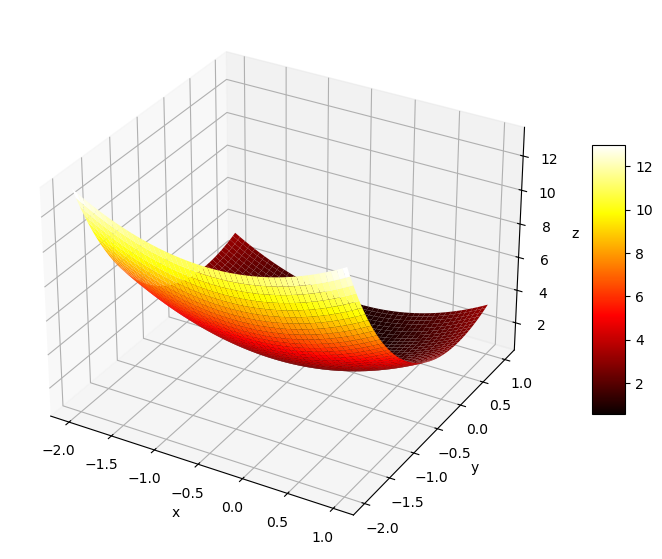
\includegraphics[width=\textwidth]{task3_surface.png}
    \caption{График $f(x)$}
\end{subfigure}
\hfill
\begin{subfigure}{0.45\textwidth}
    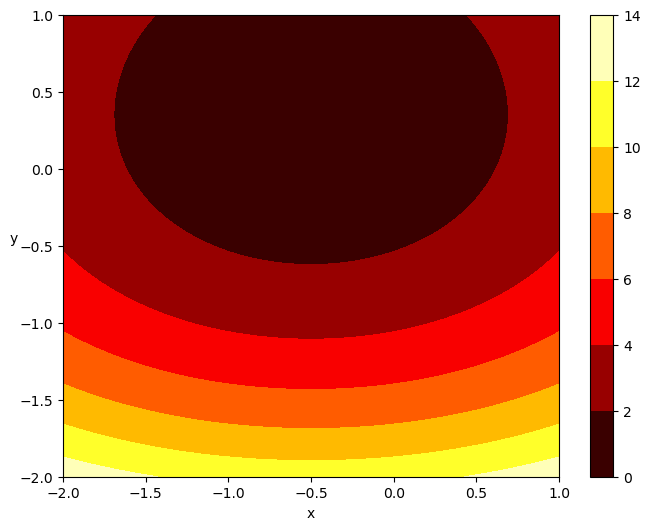
\includegraphics[width=\textwidth]{task3_contour.png}
    \caption{Поверхности уровня $f(x)$}
\end{subfigure}

\caption{Визуализация графика $f(x)$ и её поверхностей уровня на рассматриваемом прямоугольнике $[-2, 1] \times [-2, 1]. $}
\end{figure}

Из графиков видно, что в качестве начально приближения можно взять точку $(x, y) = (-0.5, 0.5)$.

\begin{table}[!h]
\centering
\begin{tabular}{|c|c|c|}
    \hline Итераций & $(x^*, y^*)$ & $f(x^*, y^*)$ \\
    \hline 3 & (-0.5, 0.35173371) &  0.57718 \\
    \hline
\end{tabular}
    \caption{Результаты нахождения точки минимума функции $f(x, y)$ на прямоугольнике $[-2, 1] \times [-2, 1]$ с помощью scipy.optimize.minimize. Погрешность найденного решенения составляет не более $10^{-6}$. В качестве начально приближения бралась точка $(x_0, y_0) = (-0.5, 0.5)$.}
\end{table}


\subsection{Код на Python}:
\begin{minted}[
frame=single,
framesep=10pt,
framerule=0.1pt,
bgcolor=LightGray
]{python}
def f(x, y):
    return x ** 2 + y ** 2 + x + np.exp(-y)

x0, x1 = -2, 1
y0, y1 = -2, 1
\end{minted}

\begin{minted}[
frame=single,
framesep=10pt,
framerule=0.1pt,
bgcolor=LightGray
]{python}
from scipy.optimize import minimize


def f_vec(x_arr: np.ndarray):
    return f(x_arr[0], x_arr[1])


x_init = np.array([-0.5, 0.5])
bounds = ((x0, x1), (y0, y1))

opt_res = minimize(f_vec, x0=x_init, tol=1e-6, 
                    bounds=bounds)
\end{minted}



\newpage
\section{Задача 9.6.10. Нахождение минимума квадратичной функции с помошью метода наискорейшего спуска}

\subsection{Формулировка задачи}
Указанным в индивидуальном варианте методом найти минимум квадратичной функции $f(x, y) = a_{11}x^2 + 2a_{12}xy + a_{22} y^2 + 2a_{13}x + 2a_{23}y$
с точностью $\varepsilon=10^{-6}$. Для решения задачи одномерной оптимизации использовать метод Ньютона. Построить график функции $f$. Предусмотреть подсчёт количества итераций, потребовавшихся для достижения заданной точности.

Согласно условию варианта минимизировать функцию необходимо с помощью \textit{метода наискорейшего спуска}, а коэффициенты равны:
\[
a_{11} = 2.5,\ \ \ 2a_{12}=-1,\ \ \ a_{22}=2,\ \ \ 2a_{13} = 0,\ \ \ 2a_{23} = -9.5 
\]

\subsection{Теоретический материал}
Предположим, что нам дана непрерывно-дифференцируемая функция $f: \mathbb{R}^n \rightarrow \mathbb{R}$ и нам необходимо решить задачу безусловной минимизации функции:
\[
f(x) \rightarrow \min\limits_{x \in \mathbb{R}^n}
\]

Одним из самых популярных методов решения данной задачи является \textit{метод градиентного спуска}. Его суть состоит в том, чтобы осуществлять оптимизацию в направлении наискорейшего убывания функции, то есть в направлении антиградиента:
\[
x_{k+1} = x_{k} - \alpha_{k} \nabla f(x_{k})
\]
Одной из вариаций градиентного спуска является \textit{метод наискорейшего спуска}, основная идея которого состоит в том, чтобы минимизировать $f(x)$ вдоль выбранного направления антиградиента:
\begin{equation}\label{steep_desc}
    f(x_k - \alpha_k \nabla f(x_{k})) =
    \min\limits_{\alpha \in \mathbb{R}}\left(
        f(x_k - \alpha \nabla f(x_k)
    \right)
\end{equation}

Метод наискорейшего спуска требует на каждом шаге решения одномерной оптимизационной задачи. Это можно делать численно, например, с помощью метода Ньютона, однако в этом случае необходимо внимательно следить за погрешностями.

В общем случае найти аналитическое решения задачи \ref{steep_desc} невозможно, однако для некоторых классов функций это сделать можно. Одним из таких классов являются квадратичные функции. Предположим, что $f(x)$ можно представить в виде
\[
f(x) = \frac{1}{2} x^T A x - b^T x + c
\]
где $A$ - положительно определённая симметричная матрица. Тогда если $\nabla f(x_k) \ne 0$, то решение оптимизационной задачи \ref{steep_desc} имеет следующий вид:
\begin{equation}\label{steep_desc:analytic}
    \alpha_k = \frac{\nabla^T f(x_k)\cdot \nabla f(x_k)}{
    \nabla^T f(x_k) \cdot A \cdot \nabla f(x_k)
    }
\end{equation}

\subsection{Порядок решения задачи}
\begin{enumerate}
    \item Решим задачу численно, то есть на каждом этапе будем решать задачу \ref{steep_desc} с помощью метода Ньютона.
    \item Решим задачу с использованием \ref{steep_desc:analytic}.
    \item Сравним результаты полученные на двух предыдущих этапах.
\end{enumerate}


\subsection{Результаты}
\begin{table}[!h]
    \centering
    \begin{tabular}{|p{1.5in}|c|c|c|c|}
    \hline \centering метод одномерной оптимизации & 
            итераций & 
            $(x^*, y^*)$ & 
            погрешность & 
            $f(x^*, y^*)$ \\
            
    \hline \centering Ньютона &
            2500 &
            (0.50003, 2.499984) &
            $2.18 \cdot 10^{-5}$ &
            -11.875 \\

    \hline \centering Аналитический & 
            10 & 
            (0.5, 2.5) & 
            $10^{-6}$ & 
            -11.875 \\
    \hline
    
    \end{tabular}
    \caption{Сравнение результатом минимизации $f(x)$ с использованием для одномерной оптимизации метода Ньютона и соотношения \ref{steep_desc:analytic}. При использовании метода Ньютона было достигнуто ограчение на число итераций, равное 2500 итераций. В качестве начального приближения бралась точка (0, 1).}
    \label{tab:my_label}
\end{table}

\newpage
\begin{figure}[!h]
\centering
\begin{subfigure}{0.45\textwidth}
    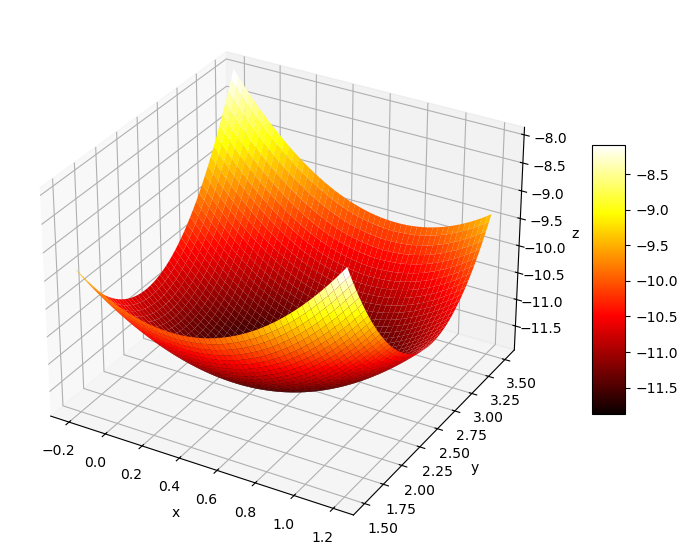
\includegraphics[width=\textwidth]{task4_surface.png}
    \caption{График $f(x)$}
\end{subfigure}
\hfill
\begin{subfigure}{0.45\textwidth}
    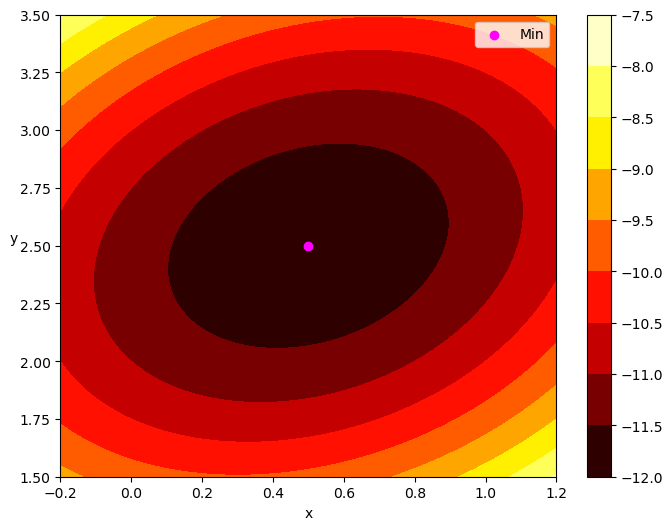
\includegraphics[width=\textwidth]{task4_contour.png}
    \caption{Поверхности уровня $f(x)$}
\end{subfigure}

\caption{Визуализация графика функции $f(x)$ и её поверхностей уровня вместе с найденной точкой минимума.}
\end{figure}


\textbf{Вывод:} Используя аналитическое решение одномерной задачи оптимизации \ref{steep_desc:analytic} нам удалось найти точку минимума с точностью $10^{-6}$. В то же время, решая одномерную задачу оптимизации с помощью метода Ньютона, нам не удалось достичь требуемой точности в силу накопления ошибки на каждом шаге.


\subsection{Код на Python}
\begin{minted}[
frame=single,
framesep=10pt,
framerule=0.1pt,
bgcolor=LightGray
]{python}
def newton_minimize(func, a0, eps=1e-6, max_iter=2500):
    func_der1 = get_der1(func)
    func_der2 = get_der2(func)

    if np.isclose(func_der2(a0), 0.0, rtol=1e-7):
        return a0
    a1 = a0 - func_der1(a0) / func_der2(a0)
    n_iter = 1
    
    while np.abs(a1 - a0) > eps:
        if n_iter == max_iter:
            return a1
        
        if np.isclose(func_der2(a1), 0.0, rtol=1e-7):
            return a1
            
        a0 = a1
        a1 -= func_der1(a1)/func_der2(a1)
        n_iter += 1
    
    return a1
\end{minted}

\begin{minted}[
frame=single,
framesep=10pt,
framerule=0.1pt,
bgcolor=LightGray
]{python}
def steepest_descent(
    A, x0, y0, opt_mode, eps=1e-6, max_iter=2500):
    """
    Minimizes the quadratic function 
    by the steepest descent method.
    """
    vec0 = np.array([x0, y0])
    g = grad_f(vec0)
    
    if np.isclose(np.linalg.norm(g), 0.0):
        return vec0, 0
    
    vec1 = vec0 - (g @ g.T) / (g @ A @ g.T) * g
    n_iter = 1

    while np.linalg.norm(vec1 - vec0) > eps:
        if n_iter == max_iter:
            error = np.linalg.norm(vec1 - vec0)
            print("Reached the iterations limit.")
            print(f"The error of the solution: {error}")
            print()
            return vec1, n_iter
        
        g = grad_f(vec1)
        vec0 = vec1.copy()
        
        if np.isclose(np.linalg.norm(g), 0.0):
            return vec1, n_iter

        if opt_mode == "analytical":
            alpha = (g @ g.T) / (g @ A @ g.T)
        elif opt_mode == "newton":
            opt_func = lambda a: f(vec1 - a * g)
            alpha = newton_minimize(opt_func, 1.0, 
                                    eps=eps * 0.1)
            
        vec1 -= alpha * g
        n_iter += 1

    return vec1, n_iter
\end{minted}


\end{document}